\documentclass[oneside]{book}
\usepackage{apjfonts}
\usepackage{geometry}
\usepackage{graphicx}
\usepackage{titletoc, titlesec}
\usepackage{hyperref}
\usepackage{geometry}
\usepackage{xcolor}
\usepackage{amsmath,mathrsfs,amsfonts}

\definecolor{main}{RGB}{0,120,2}%
\definecolor{seco}{RGB}{230,90,7}%
\definecolor{thid}{RGB}{0,160,152}%

\hypersetup{
 breaklinks,
 unicode,                
 bookmarksnumbered  =true,
 bookmarksopen      =true, 
 pdfsubject         =\@author \@title Book,
 pdfkeywords        ={ElegantBook},
 pdfcreator         ={XeLaTeX with ElegantBook class},
 colorlinks,
 linkcolor          =main,
 plainpages         =false,
 pdfstartview       =FitH,
 pdfborder={0 0 0},
 linktocpage
 }


\geometry{
    a4paper,
   left=27mm,  %% or inner=23mm
   right=27mm, %% or outer=18mm
   top=25.4mm, bottom=25.4mm,
   headheight=2.17cm,
   headsep=4mm,
   footskip=12mm
}

\titleformat{\chapter}[hang]{\Huge\bfseries}{Chapter \thechapter}{1cm}{}[]

\DeclareMathAlphabet{\mathbi}{OT1}{cmr}{bx}{it}
\SetMathAlphabet\mathbi{bold}{OT1}{cmr}{bx}{it}

\def\brains{{\texttt{brains}}}

\begin{document}

\title{\bf BRAINS:\\
Bayesian Reverberation-mapping Analysis Integrated
with Nested Sampling}
\author{Yan-Rong Li\\
Institute of High Energy Physics}

\maketitle
\tableofcontents
\mainmatter

\clearpage
\newpage

\vspace*{10cm}
{\Huge\centerline{\bf Part I: Users' Guide}}


\chapter{Installation}
\section{Third-Party Packages}
{\brains} requires the following third-party packages:
\begin{itemize}
 \item {\bf GSL}. GSL is used to generate random numbers, perform interpolation, and calculate some special functions. GSL is available at 
 \url{https://www.gnu.org/software/gsl}.
 
 \item {\bf FFTW}. FFTW is used to implement Gaussian smoothing on the line profiles. FFTW is available at \url{http://fftw.org}.
 
 \item {\bf LAPACK}. LAPACK is used to perform numerical linear algebra calculations, such as matrix operations and Cholesky decomposition.
 LAPACK is a fortran library. Its C interface is LAPACKE, included in the LAPACK package. One needs to configure the LAPACK installation
 options to switch on LAPACKE. LAPACK is available at \url{https://netlib.sandia.gov/lapack}.
 
 \item {\bf MPICH}. MPICH is a high performace and widely portable implementation of the Message Passing Interface standard.
 MPICH is available at \url{http://www.mpich.org}. 
 
 \item {\bf DNest}. DNest is a library to implement diffusive nested sampling. DNest is available at \url{https://github.com/LiyrAstroph/DNest_C}.
\end{itemize}
In popular Linux distributions, one can use the system package manager to install the above packages. For example, in Fedora distribution, 
the corresponding terminal commands are 
\begin{verbatim}
 sudo dnf install gsl fftw3 lapack mpich
\end{verbatim} 

\section{Configure the \texttt{Makefile}}
To compile {\brains}, one needs first to proporiately configure the \texttt{Makefile}.

\clearpage
\newpage

\vspace*{10cm}
{\Huge\centerline{\bf Part II: Broad-Line Region Modeling}}

\setcounter{chapter}{0}
\chapter{BLR Modeling}

\section{Coordinate rotation}
\begin{figure}[h!]
\centering
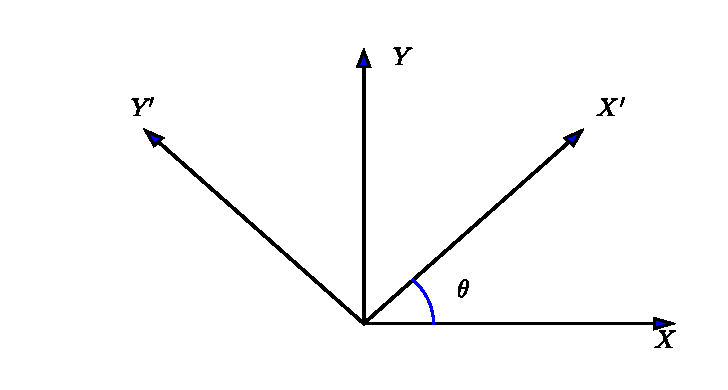
\includegraphics[width=0.5\textwidth]{coord.pdf}
\end{figure}

For the rotation of a coordinate (XOY) by an angle of $\theta$ to (X'OY'), there are relations
\begin{equation}
\left[\begin{array}{c}
\mathbi{e}_{x'} \\
\mathbi{e}_{y'}
\end{array}\right]=\left[\begin{array}{cc}
\cos\theta & \sin \theta  \\
-\sin\theta &  \cos \theta       
\end{array}\right]\left[\begin{array}{c}
\mathbi{e}_{x} \\
\mathbi{e}_{y}
\end{array}\right].
\end{equation}
and 
\begin{equation}
\left[\begin{array}{c}
\mathbi{e}_{x} \\
\mathbi{e}_{y}
\end{array}\right]=\left[\begin{array}{cc}
\cos\theta & -\sin \theta  \\
\sin\theta &  \cos \theta       
\end{array}\right]\left[\begin{array}{c}
\mathbi{e}_{x'} \\
\mathbi{e}_{y'}
\end{array}\right].
\end{equation}
Therefore, for a vector $A$, its components in (XOY) and (X'OY') are related by
\begin{equation}
A=[x', y'] \left[\begin{array}{c}
\mathbi{e}_{x'} \\
\mathbi{e}_{y'}
\end{array}\right] = [x, y]\left[\begin{array}{c}
\mathbi{e}_{x} \\
\mathbi{e}_{y}
\end{array}\right]=[x, y] \left[\begin{array}{cc}
\cos\theta & -\sin \theta  \\
\sin\theta &  \cos \theta       
\end{array}\right]\left[\begin{array}{c}
\mathbi{e}_{x'} \\
\mathbi{e}_{y'}
\end{array}\right].
\end{equation}
This yields
\begin{equation}
\left[\begin{array}{c}
x' \\
y'
\end{array}\right]=\left[\begin{array}{cc}
\cos\theta & \sin \theta  \\
-\sin\theta &  \cos \theta       
\end{array}\right]\left[\begin{array}{c}
x \\
y
\end{array}\right].
\end{equation}


In right-handed coordinate frame, we perform a rotation around $y$-axis by an angle of $l_\theta$ and 
then a rotation around $z$-axis by an angle of $l_\phi$. The transformation matrix is
\begin{equation}
\left[\begin{array}{ccc}
\cos l_\phi & \sin l_\phi & 0 \\
-\sin l_\phi &  \cos l_\phi & 0 \\
     0      &      0       & 1 
\end{array}\right]
\left[\begin{array}{ccc}
\cos l_\theta  & 0  & -\sin l_\theta\\
   0      &      1        &  0  \\
\sin l_\theta &  0  & \cos l_\theta 
\end{array}\right]=
\left[\begin{array}{ccc}
\cos l_\phi\cos l_\theta  & \sin l_\phi  & -\cos l_\phi\sin l_\theta\\
-\sin l_\phi\cos l_\theta      & \cos l_\phi        &  \sin l_\phi\sin l_\theta  \\
\sin l_\theta &  0  & \cos l_\theta 
\end{array}\right]
.
\end{equation}

\section{Time Lag}
The obsever is located at $(D\rightarrow\infty, 0, 0)$, i.e., the line of sight is along $x-$axis. 
For a cloud at $(x, y, z)$, its time lag is
\begin{equation}
\tau =\sqrt{x^2+y^2+z^2} + \sqrt{(D-x)^2+y^2+z^2} - D \approx r + D(1-x/D) - D \approx r - x,
\end{equation}
where $r=\sqrt{x^2+y^2+z^2}$.

The angle between the line of sight and the line of cloud is
\begin{equation}
 \cos \varphi = \frac{D\cdot x}{D\cdot r} = \frac{x}{r}.
\end{equation}


\end{document}

